\documentclass[letterpaper, onecolumn,10pt]{IEEEtran}

\usepackage{graphicx}
\usepackage{amssymb}
\usepackage{amsmath}
\usepackage{amsthm}

\usepackage{alltt}
\usepackage{float}
\usepackage{color}
\usepackage{url}
\usepackage{listings}
\usepackage{ifthen}


\usepackage[TABBOTCAP, tight]{}

\usepackage{geometry}
\geometry{textheight=8.5in, textwidth=6in}

%random comment

\newcommand{\cred}[1]{{\color{red}#1}}
\newcommand{\cblue}[1]{{\color{blue}#1}}

\usepackage{hyperref}
\usepackage{geometry}
\usepackage{caption}
\usepackage{url}
\usepackage{natbib}

\begin{document}
    \begin{titlepage}
    \newcommand{\HRule}{\rule{\linewidth}{0.5mm}}
    \center
    \textsc{\Large Oregon State University}\\[1.5cm]
    \textsc{\Large ST 314}\\[0.5cm]
    \textsc{\Large Summer 2019}\\[0.5cm]
    \HRule \\[0.4cm]
    { \huge \bfseries Data Analysis Seven}\\[0.4cm] % Title of your document
    \HRule \\[1.5cm]
    \begin{minipage}{0.4\textwidth}
        \begin{flushleft} \large
        \emph{Author:}\\
        Thomas Noelcke
        \end{flushleft}
    \end{minipage}
    \begin{minipage}{0.4\textwidth}
        \begin{flushright} \large
        \emph{Instructor:} \\
        Katie Jager\\
        \end{flushright}
    \end{minipage}\\[2cm]
		\end{titlepage}
        
        \section{Part 1}
            \subsection{}
            %Include Graphics here
            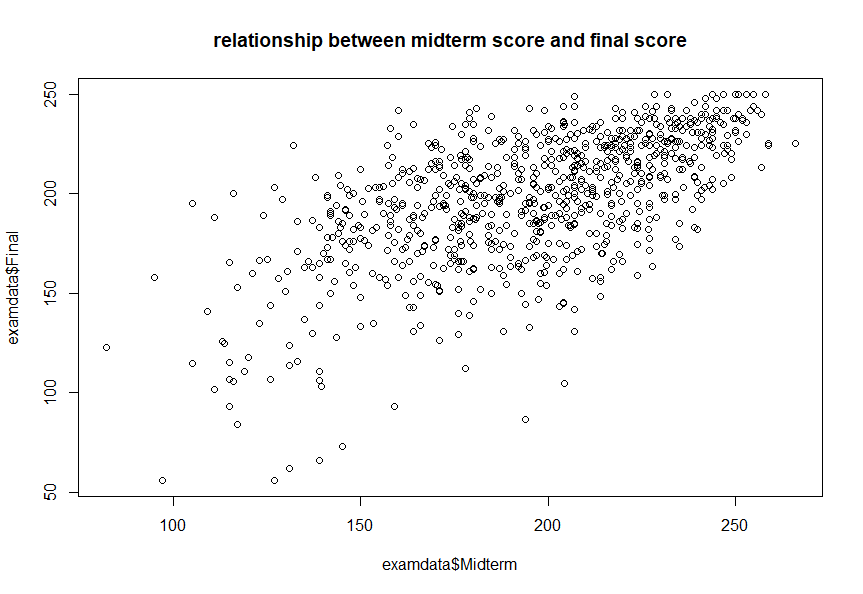
\includegraphics[width=\textwidth]{Week7/Images/scatterplot.png}
            
            The plot above shows the relationship between Midterm Exam Score (x) and Final Exam Score (y). There does appear to be a relationship between midterm score and final score. However I would consider this relationship weak as it doesn't seem to focus around a single line. The relationship between midterm score and final score has positive slop. This means that people who score well on midterms tend to score well on the final on average.\\
            
            \subsection{}
            Using R I calculated the correlation coefficient and determined that it was 0.6165. This does support my assertion that the relationship between final score and midterm score is positive. However, I previously said that the strength was weak when I should have said that it was moderate.\\
        
        \section{Part 2}
            \subsection{}
            Below is the result of running the R command to calculate the least squares regression.
            \begin{lstlisting}
                 Estimate Std. Error t value Pr(>|t|)    
(Intercept)      82.90643    5.14771   16.11   <2e-16 ***
examdata$Midterm  0.58644    0.02595   22.60   <2e-16 ***
            \end{lstlisting}
            Below is the least squares regression line.
            
            \[
                0.58644x + 82.90643
            \]
            
            \subsection{}
            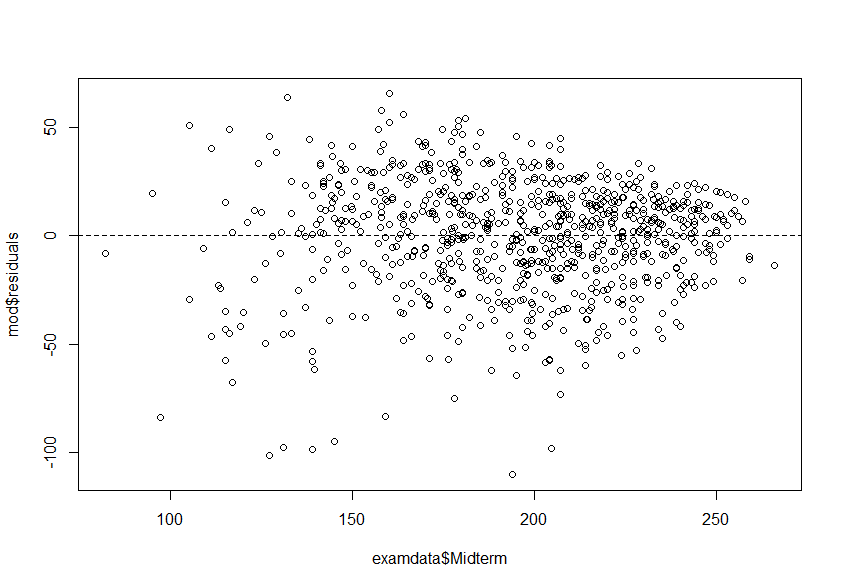
\includegraphics[width=\textwidth]{Week7/Images/residuals.png}
             
             Above is the plot of the residuals from the calculation in step one. While looking at the plot I found that the relationship did not violate the linearity assumption. However, Looking at the data it seems that this relationship may violate the constant variation assumption as the data seems to follow a pattern with a cone where the residuals are focused around two lines. There is also an issue with the distribution of the residuals. The pattern does not seem totally random and there are more negative values than positive values. This means that this relationship violates the normality assumption.\\
        
        \section{Part 3}
            \subsection{}
            The null and alternative hypothesis are stated below.
            
            \[
                H_0 = \beta_1 = 0
            \]
            \[
                H_a =  \beta_1 \neq 0
            \]
            
            \subsection{}
            The test statistic for the relationship from the output in part 2 as as follows, The F-stat is 510.8 and the P-Value is 2.2e-16 or ~0. The degrees of freedom are 833.\\
            
            \subsection{}
            There is convincing evidence that midterm score is a significant predictor of final exam score. We reject the null hypothesis at a significance level of 0.05(f = 510.8, p-value = 2.2e-16)\\
            
            \subsection{}
            The calculation for the 95\% interval for the slope of the relationship between midterm exam scores and final exams scores is shown below.
            
            \[b_1 \pm t^*XSE_{b1}\]
            \[SE_{b1} = 0.02595, t^* = 1.9628\]
            \[ 0.58644 \pm 1.9628*0.02595\]
            \[= [0.5355, 0.6373]\]
            
            There is a 95\% chance that the true slope of the relationship between midterm exam score and final exam score is between 0.5355 and 0.6473 with a point estimate of 0.5864.\\
        \section{Part 4}
            \subsection{}
            Shown below is a prediction of the final exam score for a student that scored 172 on the midterm using the line we found in part 2a.
            
            \[f_{score} = m_{score}*0.58644 + 82.90643\]
            \[f_{score} = 172*0.58644 + 82.9043 = 183.767\]
            
            \subsection{}
            Our prediction for the final exam score was 183.767 where as the student actually score 162.5. The model predicted that the exam score would be to high with a residual of 21.267\\
            
            \subsection{}
            The prediction interval is 133.35, 234.20 where as the confidence interval is 181.66, 185.89 because the prediction interval is always wider than the confidence interval.\\
            
            \subsection{}
            The interval that will represent the final exam prediction will be the 133.35 to 234.20 interval because we are making a prediction about a single person where we must factor in much more uncertainty.\\
            
            \subsection{}
            My midterm grade was 218. Based on my midterm grade I've calculated my final grade below.
            
            \[
                218*0.58644 + 82.90643 = 210.75
            \]
            
            \subsection{}
            For my case I think that the prediction is not reasonable. This is mostly due to some lurking variables that the model couldn't possibly deal with like the fact that I currently own two houses and am trying to get one of them sold and as such have not studied all that well. I also think that the strength of the model lends it self to large variance in the prediction vs the actual outcome. We can see this in the prediction outcome above.\\
            
		\end{document}